	\section{OTP Platform}

La concorrenza sembra gestita quasi come un gioco in Elixir,
ma ciò in genere non basta per semplificare lo sviluppo
di un software, per questo Elixir supporta l'insieme di
librerie OTP sviluppate per Erlang, con un Api più pulita
e moderna rispetto al suo predecessore.
L'OTP (Open Telecom Platform) è un insieme di librerie,
strumenti e linee guida per sviluppare dei sistemi
scalabili e resilienti in Erlang ed
Elixir, basti pensare che per via dell'immutabilità
dei dati e della natura funzionale del linguaggio,
non possiamo avere variabili globali che mantengono
uno stato, e per fare ciò, Elixir consente di dare
la responsabilità nel mantenimento di uno stato
ad un processo. Astrazioni come l'\textbf{Agent} o il \textbf{GenServer}
ci consentono di mantenere uno stato senza dover reinventare la
ruota nello scrivere un modulo soltanto per mantere un semplice stato.
L'approccio nella programmazione è totalmente differente
e piuttosto singolare rispetto ai più comuni linguaggi di programmazione,
ma è proprio questa singolarità che può portare dei vantaggi in alcune
nel mondo concorrenziale. 

%---------------------------------------------------------------------------------

\subsection{GenServer}
Si può volere più controllo rispetto alle primitive utilizzate
per gestire la concorrenza, un OTP server è un modulo con il
"Behaviour" GenServer. 
Il "Behaviour" è un meccanismo che consente di definire
uno schema comune per un tipo specifico di processo.

Ad esempio il GenServer Behaviour definisce le funzioni e
le interfacce necessarie per creare un processo server in grado
di gestire le richieste in modo asincrono.
Utilizzando il GenServer Behaviour, è possibile definire i comportamenti
di base del server e personalizzarli secondo le esigenze specifiche
dell'applicazione. 
Questo fornisce un alto livello di astrazione per la gestione
dei processi e semplifica lo sviluppo di sistemi concorrenti e
distribuiti in Elixir.

Il vantaggio di utilizzare un GenServer è che ha un'insieme
di interfacce standard e include funzionalità di tracciamento
e segnalazione degli errori. Si può anche mettere dentro un
albero di supervisione.

Questo Behaviour astrae l'interazione Client-server, come si può vedere
in figura \ref{fig:client_server}  \cite{GenServe6:online}.

\begin{figure}[!htp]
    \centering
    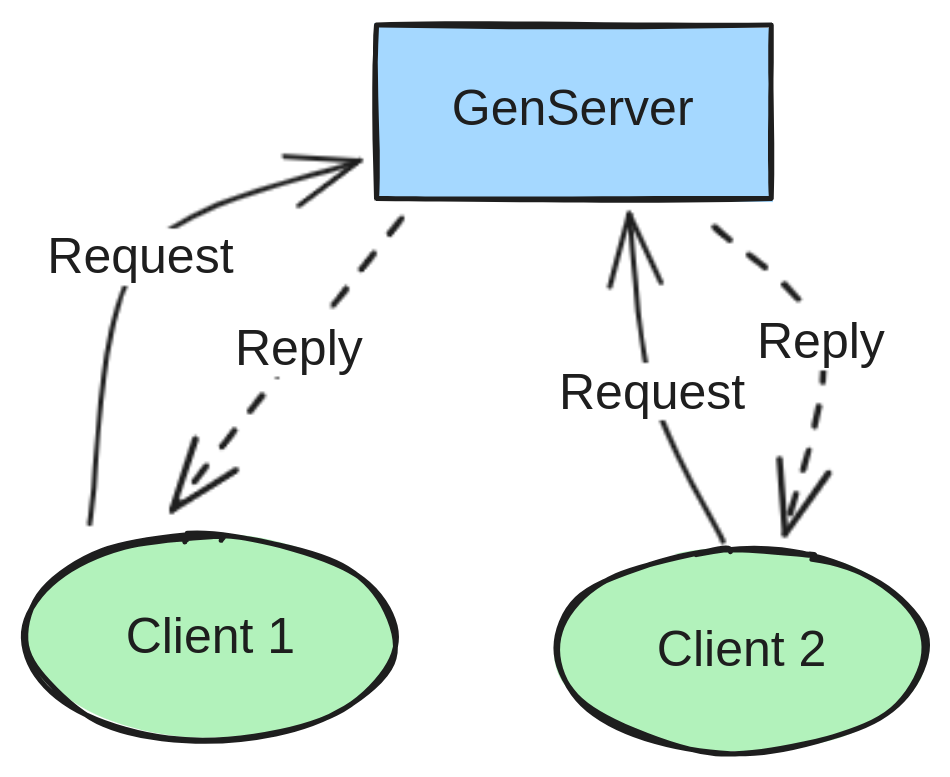
\includegraphics[keepaspectratio=true,scale=0.20]{images/GenServer.png}
	\caption{Interazione Client-Server}
  	\label{fig:client_server}
\end{figure}

Per implementare il behaviour GenServer, bisogna affidarsi alla
documentazione di GenServer, in particolare vanno ridefinite delle
callback, ed ogni funzione può restituire un determinato insieme di
strutture dati.

Nell'esempio \ref{lst:stackGenServer} viene implementata una struttura dati
per mantere uno Stack di dati \cite{GenServe6:online}.

\begin{lstlisting}[language=elixir, caption={Implementazione Stack},captionpos=b,
	label={lst:stackGenServer}]
defmodule Stack do
use GenServer

# Client

def start_link(default) when is_binary(default) do
  GenServer.start_link(__MODULE__, default)
end

def push(pid, element) do
  GenServer.cast(pid, {:push, element})
end

def pop(pid) do
  GenServer.call(pid, :pop)
end

# Server (callbacks)

@impl true
def init(elements) do
  initial_state = String.split(elements, ",", trim: true)
  {:ok, initial_state}
end

@impl true
def handle_call(:pop, _from, state) do
  [to_caller | new_state] = state
  {:reply, to_caller, new_state}
end

@impl true
def handle_cast({:push, element}, state) do
  new_state = [element | state]
  {:noreply, new_state}
end
  end
\end{lstlisting}

Nell'esempio possiamo vedere che il modulo stack implementa
la funzione \textbf{init/1} che inizializza lo stato con gli elementi
iniziali quando il server viene avviato, la funzione \textbf{handle\_call/3}
chiamata per le operazioni di :pop dello stack, in particolare
è una funzione sincrona, quindi viene usata quando ci si aspetta
un valore di ritorno, infatti restituisce il valore di
testa dello stack. La funzione \textbf{handle\_cast/2} invece viene usata per
le operazioni asincrone, quindi nel caso in esame per l'operazione di
push nello Stack.

Quindi il GenServer è un'astrazione che:

\begin{itemize}
	\item Incapsula un servizio condiviso.
	\item Mantiene uno stato.
	\item Permette un'astrazione concorrente ad un servizio condiviso \cite{adoptingElixirchap5pag96}.
\end{itemize}

%---------------------------------------------------------------------------------

\subsection{Supervisor}

Un Supervisor è un modulo che implementa il Behaviour Supervisor,
sono processi specializzati per un solo scopo: monitorare altri processi
che chiameremo d'ora in poi processi figli.

Sono questi Supervisor che ci semplificano lo sviluppo di applicazioni
fault-tolerant, supervisionando i processi figli.
Bisogna quindi decidere quali sono i processi figli da supervisionare,
e una volta avviato il Supervisor con la funzione \textbf{start\_link/2},
questo ha bisogno di sapere come avviare, fermare o riavviare i suoi figli
in caso di errore o uscita imprevista.

Per questo i figli hanno bisogno di avere una funziona \textbf{child\_spec/1}
che definisce il comportamento del supervisore. I moduli che implementano
lo GenServer, oppure un Agent automaticamente definiscono questa funzione,
quindi non c'è bisogno di modificare il modulo.
La funzione child\_spec/1 è una funzione che restituisce una Map per
configurare il comportamento in caso di supervisione.

